\documentclass[12pt]{article}


%-=-=-=-=-=-=-=-=~TODO~-=-=-=-=-=-=-=-=

% ?DONE? Update table formatting

%% Clearly State the Objective: What is happening in the class beforehand i.e. why are we doing this?

%% Add more examples of prior work
%% More detail on peer instruction

%% Describe plickers more 
%% Update to include text of Zoom questions

%% Describe the process in the classroom
%%% i.e. Question presented, students respond, students write down answer, check results, if < 80% redo, else continue
%% At what point do students write down the question and answers. Is this within the alotted time to answer and discuss? How may this impact the results?

%% Add demographic data if possible

%% Update language around Zoom v. In-person
%%% Section 5 suggests that the students may have done better remotely. What evidence is there for this? Could that be suggestive that plickers are a hinderance, or is it more suggestive that online technologies are superior, etc?


%% Typos:
%%% Evidence: typo 61.35% vs 57.35%


%%?? Add Sections for: discusion, Conclusion, threats to validity 


%-=-=-=-=-=-=-=-=-~Packages~=-=-=-=-=-=-=-=-=-=-=
\usepackage[english]{babel}
% \usepackage[utf8x]{inputenc}
\usepackage{amsmath}
\usepackage{graphicx}
\graphicspath{ {./images/} }
\usepackage{etoolbox}
\usepackage{changepage}
\usepackage{titlesec}
\usepackage[parfill]{parskip}
\usepackage[margin=1in]{geometry}
\usepackage{times}
\usepackage{float}
\usepackage{csquotes}
% \usepackage[numbers,super]{natbib}
\usepackage{lipsum} % Package to generate dummy text throughout this template. Remove for real use.

% \usepackage{biblatex}
\usepackage{color, colortbl}

\usepackage{graphicx}
\graphicspath{ {./images/} }
\usepackage{booktabs}
\usepackage{url}
\usepackage{geometry}
\usepackage{pdflscape}
\usepackage{multicol}
\usepackage{calculator}

%-=-=-=-=-=-=-=-=-~Variables~=-=-=-=-=-=-=-=-=-=-=
\newcommand\sampleSize{163}
\newcommand\classSize{269}


%% Color Definitions
\definecolor{LightGray}{gray}{.8}

%----------------------------------------------------------------------------------------
%  TITLE SECTION
%----------------------------------------------------------------------------------------

\titleformat*{\section}{\normalsize\bfseries} % Makes section titles 12 pt font

\title{\large \textbf{Plickers and Peer Instruction in a Software Design Course}} % using \large makes the title approximately 14 pt.
% Author info isn't included for the Annual Conference but some regional conferences might request it.
%%\author{}
\author{\normalsize}
\date{} % This leaves the date blank.

\makeatletter % This gets the margins for the title set.
\patchcmd{\@maketitle}{\begin{center}}{\begin{adjustwidth}{0.5in}{0.5in}\begin{center}}{}{}
\patchcmd{\@maketitle}{\end{center}}{\end{center}\end{adjustwidth}}{}{}
\makeatother

%----------------------------------------------------------------------------------------

\begin{document}
% \raggedright
\maketitle
\thispagestyle{empty}
\pagestyle{empty}

%----------------------------------------------------------------------------------------
%  PAPER CONTENTS
%----------------------------------------------------------------------------------------
\section*{Abstract}
Active learning strategies, such as peer instruction, have been shown to increase student achievement in STEM classes.  This  paper explores a case study of peer instruction with direct student feedback using printed response cards (Plickers) or Zoom polls.

Combining peer instruction with Plickers provides instructors and students with timely feedback on course material.  This feedback allows instructors to gauge which topics students have understood and which may need more explanation or practice.  Additionally the use of peer instruction provides students with multiple perspectives on challenging topics.  This paper examines how these tools are used to provide instruction to students where it is needed most in a scalable and relatively low effort way.  

Students were polled once or twice per class meeting and responded with either Plicker cards (for in-person classes) or Zoom polls (for remote classes). Peer instruction was used  when the initial poll resulted in a low percentage of correct answers; pre-selected student groups  discussed the question for a set amount of time, after which students.  Peer instruction allowed students to get real time feedback on topics that needed more coverage and allowed the instructor insight into students comprehension.

Data were collected in a junior level computer science software design course over four semesters with an overall n of \sampleSize. The course ran for two hours, twice a week. 

The data collected indicate that students found peer instruction to be helpful in their understanding of the material.  Similarly, students reported that the use of peer instruction helped them pay attention and that it was a valuable tool in learning the material.  Zoom polls worked well during remote instruction and may be a viable option for remote learning.  

After the initial effort in creating the question banks used for polls this process takes very little extra work and provides valuable insight to the instructor and students.  Calling on students to explain answers allows further insight into student understanding.  The  additional instruction helps students to engage with their peers and to better understand the material.  Future work will focus on comparing the pre and post poll responses and in improving group discussion and interaction.
 
\section{Introduction}
Peer instruction has long been an effective strategy to improve student performance in STEM classes ~\cite{porterMultiinstitutionalStudyPeer2016} ~\cite{porterHalvingFailRates2013} ~\cite{simonExperienceReportPeer2010a}. One limiting factor to the implementation of peer instruction is the cost associated with purchasing clickers.  This can be especially prohibitive for smaller institutions.  
This report examines the use of peer instruction with the free online tool Plickers \url{https://www.plickers.com/} and Zoom online polls during remote instruction.  
This implementation of peer instruction is directly modeled from the work of Leo Porter ~\cite{porterMultiinstitutionalStudyPeer2016}.  The typical model presents students with a multiple-choice question (MCQ). If the percentage of correct answers fall below a threshold students then discuss the question in groups. Once a predetermined amount of time has passed students once more answer the question.

In this report we examine the existing literature on peer instruction and the peer instruction model that inspired this work.  We also report on updating and using peer instruction during remote instruction.  We also discuss possible improvements to the intervention, such as ways to increase student interaction and better question design. The goal of this intervention was to increase student engagement in the material and to build a library of questions to represent the key concepts in the course. 

In the next section, we examine the literature relating to peer instruction and how it may improve student performance.  We also explore variations on peer instruction implementation and question design. 

\section{Supporting Literature}
First we present supporting work in peer instruction.  Then we discuss active learning, including its limitations. 

\subsection{Peer Instruction}
Peer instruction has been used in science education since at least 1990 ~\cite{crouchPeerInstructionTen2001}. In that time it has been shown to increase student performance and to be an effective way to engage students in challenging material ~\cite{simonExperienceReportPeer2010a} ~\cite{porterMultiinstitutionalStudyPeer2016}. Though much of the work on peer instruction in computer science (CS) focuses on introductory classes, there has been some work that shows that peer instruction is effective in upper division courses as well ~\cite{leeCanPeerInstruction2013}.
The major influence for this work is the peer instruction model described in \cite{porterPeerInstructionStudents2011}. This model is primarily used in introductory computer science courses (CS1) courses but was adapted here for junior level students. 

\subsection{Active Learning}
In the 2014 Freeman report, published in the proceedings of the National Academy of Science, the authors performed a meta-analysis of 225 studies and found that active learning boosted test scores and lowered failure rate in science, technology, and engineering (STEM) classes ~\cite{freemanActiveLearningIncreases2014}. In a 2012 presidential report titled ``Engage to Excel'' there was a call for one million additional STEM graduates and a recommendation to use active learning as a way to meet this goal ~\cite{gatesEngageExcel2012}. These reports also indicate a disproportionately positive impact of active learning on under represented minority students ~\cite{freemanActiveLearningIncreases2014}.
In a meta-analysis from 2004, Prince cautions faculty that simply adopting an active learning approach is no guarantee of success ~\cite{princeDoesActiveLearning2004}. However, the author concluded that: ``Although the results vary in strength, this study has found support for all forms of active learning examined''. Prince goes on to state that among the most effective forms of active learning are those that involve collaboration and group learning activities.
Active learning is further supported by Bloom’s Taxonomy, which suggests moving lower level instruction and cognitive tasks outside of class time has a beneficial effect on recall and concept retention ~\cite{andersonTaxonomyLearningTeaching2014}. Students being responsible for lower level procedural learning outside of the classroom will also make room for instructors to focus on problem solving and meaningful dialog in the classroom.


\section{Background}

Here we describe the structure of the course where there intervention took place. Then we describe the tools that were used as well as the modifications made during remote instruction. Finally, we discuss the specific implementation of peer instruction covered in this report.

\subsection{Course Description}
This study examines an upper-division software design course taught in Java. The course takes place at a small public North American university on a 16 week semester system. Students enrolled in this course have one or two semesters of programming experience. About half of the students in the course are transfers from other institutions, typically local community colleges. The non-transfer students do not have experience with Java. 
In this report we examine courses taught between Spring 2020 – Spring 2021 and Spring 2022 – Fall 2023.  The researcher did not teach the course during the Fall 2021 semester so no data were collected \. Enrollment by semester is shown in table ~\ref{table:enrollmentBySemester}.

Typically this course has a high drop, fail, withdraw rate (DFW).  This course is also one of the first programming classes taken by transfer students.

% \DIVIDE{\sampleSize}{\classSize}{\sol}
% \DIVIDE{\sampleSize}{\classSize}{\sol}
% \ROUND[2]{\sol}{\sol}
% $6/7=\sol$\%

\begin{table}[ht]
\centering
\caption{Enrollment per semester}
\begin{tabular}{|c|c|c|}
\toprule
Semester    & n  & sections\\ \midrule
\rowcolor{LightGray}
Spring 2020 & 70 & 2 \\ \midrule
Fall 2020   & 43 & 1 \\ \midrule
\rowcolor{LightGray}
Spring 2021 & 70 & 2 \\ \midrule
Spring 2022 & 57 & 2 \\ \midrule
\rowcolor{LightGray}
Fall 2022 & 29 & 1 \\ \midrule
Totals & \classSize & 8 \\ \bottomrule
\end{tabular}
\label{table:enrollmentBySemester}
\end{table}

\begin{table}[ht]
\centering
\caption{With which gender identity do you most identify?}
\begin{tabular}{|c|c|}
\toprule
Another gender identity & 1 \\\midrule
\rowcolor{LightGray}
Female & 35 \\\midrule
Male & 118 \\\midrule
\rowcolor{LightGray}
Prefer not to answer & 3\\\midrule
Did not answer & 6\\ \bottomrule
\end{tabular}
\end{table}

\subsection{Plickers}
``Plickers'' (\url{https:\\www.plickers.com}) \footnote{The authors have no connection to Plickers or the company that creates the service.} is an online service that allows students to respond to a multiple-choice question presented in class. Students raise a printed card and orient it such that their answer choice is at the top of the card. The instructor uses a mobile device with a camera to scan the cards and get a real time report of the student answers. Students see when their responses are recorded however the specific answer is only visible to the instructor. The results of the student choices are stored, and the instructor may review them later. The application does not store images of the students, only the result of scanning the cards. 

\begin{figure}[ht]
  \centering
  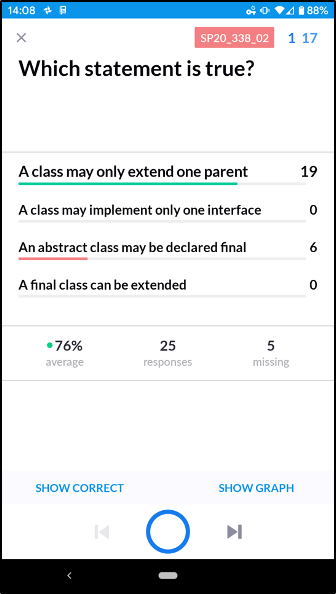
\includegraphics[]{instructor_view.png}
  \caption{The instructor view of a question on a mobile device.}
  % \Description{Instructor view of a mobile device}
  \label{fig:plicker_instructor_view}
\end{figure}

Plickers offer a few advantages over traditional clickers for recording student responses. The overall cost is low, the cards may be printed from home on standard printer paper. In the event that a student forgot their plicker, the instructor had a full set of spare cards. The spare cards were only made available during the first three weeks, after which it was the students responsibility to print their own replacement card. Students are also able to use devices such as mobile phones and tablets to have an electronic version of their card.  In some cases students even used their laptop computer to display their cards.

% \begin{multicols}{2}

\begin{figure}[ht]
  \centering
  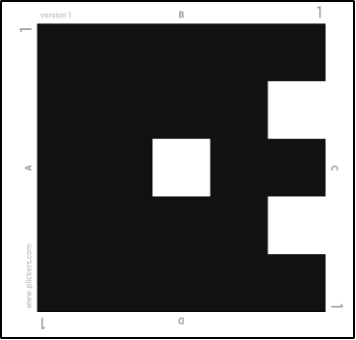
\includegraphics[width=50mm,scale=0.5]{plicker_card.png}
  \caption{Example Plicker Card.}
  % \Description{Example Plicker Card}
  \label{fig:plicker_card}
\end{figure}
\begin{figure}[ht]
  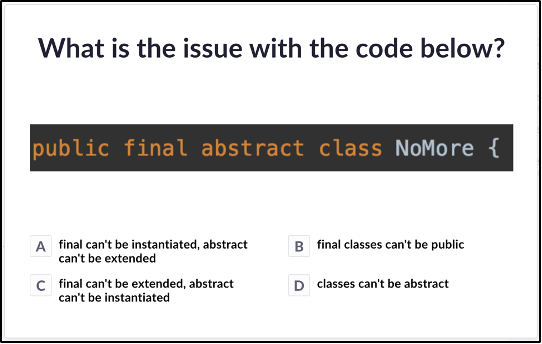
\includegraphics[width=\linewidth]{plicker_question.png}
  \caption{Example Plicker Question Before the Correct Answer is Shown.}
  % \Description{Example Plicker Question Before the Correct Answer is Shown.}
  \label{fig:plicker_question}
\end{figure}

% \end{multicols}

\subsection{Peer Instruction Implementation}

As discussed earlier the peer instruction model followed here adapted from the work of Leo Porter \cite{porterPeerInstructionStudents2011}. The implementation differed from the work of Porter in a few key areas. Notably in Porter`s implementation the elapsed time is shown while students respond to the questions, in this implementation students were given a time limit on both the initial, and any follow up, questions. 

Another difference is the use of Plickers rather than more traditional clickers. Plickers, and their use, are discussed in the next section.

Generally, at two points during the class session, students were presented with multiple choice questions. Questions were shown on the projector and students had between 60-90 seconds to think about the question on their own before answering with the Plicker cards. If more than 90\% of the class got the question correct, the correct answer was shown and a brief explanation was given. If the percentage of correct responses was below 90\% students were given 90–120 seconds to discuss the question with their assigned groups before answering the questions again. The instructor would prompt students on what to discuss, or remind them about when the topic had been discussed in class. 

After the group discussion the correct answer is displayed and students are asked to explain why the other answers were incorrect. This allowed for more detail on the question and demonstrated critical reasoning. The mobile Plicker application displays which students had correct answers so these students were chosen to explain why they did not choose the incorrect answers. These students were selected because the instructor did not wish to single out students who got the question wrong.

An addition to the peer instruction model being followed here is the requirement that students write down the questions and their answers to them. The instructor emphasizes that writing down the question and all the answers, correct or otherwise, is important to their learning \cite{metcalfeMemoryTruthCorrecting2019}. At the end of each class sessions students must turn in a PDF document with their individual answers as well as the answer arrived at after group discussion. Students were also instructed to write down why any of their answers were incorrect. This leads to the normalization of answering a question incorrectly and encourages students to think critically about how to identify correct and incorrect answers.


\subsection{Zoom and remote learning}
During the later half of the Spring 2020 semester and the entire Fall 2020 semester, instruction was fully remote due to the COVID-19 pandemic. The meeting software ``Zoom''  was used during this time. Zoom offers a polling feature that allowed students to answer multiple choice questions in the same way Plickers were used in person. In order to use Zoom polls questions were shown on a slide deck rather than through the Plicker website. Since the polling feature was somewhat limited, and given time constraints, the same multiple choice poll was used for all of the questions. 
Zoom allows for the creation of ``breakout rooms'' to allow students to discuss questions in small groups. Students were randomly sorted into groups that would persist for 2–3 weeks before being randomized again. While students were in breakout rooms, the instructor would visit to clear up any issues and ensure students were discussing the question. These tools allowed for the continued use of peer instruction during remote instruction and in some ways were more successful than in-person instruction.

\section{Results}

Student perception of the use of Plickers was measured with a questionnaire that was administered at the end of each semester. In total there were seven sections across four semesters as shown in table ~\ref{table:enrollmentBySemester}. In total there were \sampleSize responses to the questionnaire for a response rate of 56.67\%.

The questionnaire was comprised of 25 questions adapted, with permission, from the work of Leo Porter ~\cite{porterPeerInstructionStudents2011}. The questionnaire consisted of: 16 Likert scale questions on a five-point scale; one likert-scale question on a four-point scale;  two free response questions; and six demographic questions. 

Table ~\ref{table:questionnairesummary} presents a summary of nine of the questions relating to the use of Plickers/Zoom Polls and peer instruction in the class. All but the last question are coded so that ``Strongly Disagree'' is the most negative and ``Strongly Agree'' is the most positive answer. The final question listed in table ~\ref{table:questionnairesummary} is coded so that ``Strongly Disagree'' is the most positive answer and ``Strongly Agree'' is the most negative answer. Note also that during online instruction the questionnaire asked about Zoom polls rather than Plickers.
\begin{landscape}
\begin{table*}[ht]
\caption{Sample Questionnaire Results.\\\hspace{\textwidth}(SD=Strongly Disagree, D=Disagree, N=Neither Disagree nor Agree, A=Agree, SA=Strongly Agree, U=Unanswered)}
% \begin{tabular}{p{0.45\linewidth} |c|c|c|c|c|c} % {l}eft {c}enter {r}ight
\begin{tabular}{p{0.25\linewidth} |c|c|c|c|c|c} % {l}eft {c}enter {r}ight
\toprule
Question Text & SD & D & N & A & SA & U\\\midrule
\rowcolor{LightGray}  %q26
Discussing Plicker questions with my classmates helped me learn the course material. & 6 (3.68\%)& 3 (1.84\%) & 18 (11.04\%) & 75 (46.01\%)& 55 (33.74\%) & 6 (3.68\%)\\\midrule
%q11
Plickers with discussion is valuable for my learning. & 0 (0\%)& 2 (1.23\%) & 13 (7.98\%) & 85 (52.15\%)& 57 (34.97\%) & 3 (3.68\%)\\\midrule
\rowcolor{LightGray} %q9
Plickers are an easy-to-use class collaboration tool. & 0 (0\%)& 3 (1.84\%) & 3 (1.84\%) & 72 (44.17\%)& 79 (48.47\%) & 6 (3.68\%)\\\midrule
%q10
Plickers helped me pay attention in this course compared to traditional lectures. & 1 (0.61\%) & 1 (0.61\%) & 14 (8.59\%) & 82 (50.31\%)& 59 (36.20\%) & 6 (3.68\%)\\\midrule
\rowcolor{LightGray} %q8
Generally, by the time we finished with a question and discussion, I felt pretty clear about it. & 1 (0.61\%)& 4 (2.45\%) & 21 (12.88\%) & 104 (63.80\%)& 27 (16.56\%) & 6 (3.68\%)\\\midrule
%q12
I recommend that other instructors use this approach (reading quizzes, Plickers, in-class discussion) in their courses. & 0 (0\%)& 1 (0.61\%) & 15 (9.20\%) & 87 (53.37\%)& 53 (32.52\%) & 7 (4.29\%))\\\midrule
\rowcolor{LightGray}%q6
The immediate feedback from Plickers helped me identify gaps in my knowledge about the course. & 3 (1.84\%) & 3 (1.84\%) & 4 (2.45\%) & 63 (38.65\%)& 84 (51.53\%)& 6 (3.68\%)\\\midrule
%q5
Most of the time my group discusses the Plicker question.  & 6 (3.68\%) & 12 (7.36\%)& 21 (12.88\%)& 63 (38.65\%)& 53 (32.52\%)& 8 (4.91\%)\\\midrule
\rowcolor{LightGray} %q7
Knowing the right answer is the only important part of the Plicker question. & 26 (15.95\%) & 85 (52.15\%)& 23 (14.11\%)& 15 (9.20\%)& 7 (4.29\%) & 7 (4.29\%)
\\\bottomrule
\end{tabular}
\label{table:questionnairesummary}
\end{table*}
\end{landscape}
\restoregeometry

The questions shown in table ~\ref{table:timeForQuestions} were used to measure the student`s opinion of the amount of time given for reading and answering multiple choice questions and the amount of time allotted to group discussion. Over 85\% of the responding students felt the time given to read the questions was appropriate. Over 80\% of the responding students felt there was an appropriate amount of time for group discussion. 

\begin{table*}[ht]
%q14
\caption{Time for reading and answering questions\\\hspace{\textwidth} (ML=Much Too Long, TL=Too long, AR=About Right, TS=Too Short, MS=Much Too Short, U=Unanswered)}
\begin{tabular}{p{0.25\linewidth} |c|c|c|c|c|c} % {l}eft {c}enter {r}ight
\toprule
Question Text & ML & TL & AR & TS & MS & U \\ \midrule
\rowcolor{LightGray}%q14
In general, the amount of time to read and understand the questions before the first vote was & 1 (0.61\%) & 7 (4.29\%) & 137 (84.05\%) & 9 (5.52\%) & 2 (1.23\%) & 5 (3.07\%) \\ \midrule %q16
The amount of time generally allowed for peer discussion was & 1 (0.61\%) & 19 (11.66\%) & 129 (79.14\%) & 7 (4.29\%) & 0 (0\%) & 5 (3.07\%) \\ \bottomrule
\end{tabular}
\label{table:timeForQuestions}
\end{table*}

As stated earlier in the paper, students did not always discuss the question in their group. Table ~\ref{table:groupDiscussion} shows that only 61.35\% of the student respondents answered that they always discussed the question in their group. Many of the students, 35.29\%, said they sometimes discussed the question. 

\begin{table}[ht]
\caption{Which of the following best describes your discussion practices in the class this term?}
\begin{tabular}{p{0.55\linewidth}|c} % {l}eft {c}enter {r}ight
\toprule
 \rowcolor{LightGray}  %q15
 I always discuss with the group around me, it helps me learn & 80 (49.08\%)\\\midrule 
 I always discuss with the group around me, I don't really learn, but I stay awake & 15 (9.20\%)\\\midrule 
 \rowcolor{LightGray}
 I sometimes discuss, it depends & 53 (32.52\%)\\\midrule 
 I rarely discuss, I don't think I get a lot out of it & 5 (3.07\%)\\\midrule 
 \rowcolor{LightGray}
 I rarely discuss, I'm too shy & 3 (1.84\%)\\\midrule 
 Unanswered & 5 (3.07\%)\\\bottomrule 
\end{tabular}
\label{table:groupDiscussion}
\end{table}

When asked about their comfort level discussing questions the majority of students, 75.73\%, claimed to be either slightly or extremely comfortable talking with their classmate. This information is show in table ~\ref{table:group_comfort}.

%comfort q28
\begin{table}[ht]
\caption{How comfortable were you talking with your classmates?}
\begin{tabular}{p{0.55\linewidth}|c} % {l}eft {c}enter {r}ight
\toprule
 \rowcolor{LightGray} 
 Extremely uncomfortable & 1 (0.61\%)\\\midrule 
 Slightly uncomfortable & 13 (7.98\%)\\\midrule 
 \rowcolor{LightGray}
 Neither comfortable nor uncomfortable & 20 (12.27\%)\\\midrule 
 Slightly comfortable & 57 (34.97\%)\\\midrule 
 \rowcolor{LightGray}
 Extremely comfortable & 65 (39.88\%)\\\midrule 
 Unanswered & 5 (3.07\%)\\\bottomrule 
\end{tabular}
\label{table:group_comfort}
\end{table}

Table ~\ref{table:questionDifficulty} shows the summary information about student perceptions of question difficulty. The single most common answer was ``Neither Too Hard Nor Too easy'' at 88.24\%. 

\begin{table}[ht]
\caption{From the perspective of helping me learn, the content of Plicker questions was}
\begin{tabular}{p{0.55\linewidth}|c} % {l}eft {c}enter {r}ight
% \toprule
 \rowcolor{LightGray} 
 Much Too Hard & 0 (0\%)\\\midrule 
 Too Hard & 0 (0\%)\\\midrule 
 \rowcolor{LightGray}
 Neither Too Hard nor Too Easy & 139 (85.28\%)\\\midrule 
 Too Easy & 15 (9.20\%)\\\midrule 
 \rowcolor{LightGray}
 Much Too Easy & 2 (1.23\%)\\\midrule 
 Unanswered & 5 (3.07\%)\\\bottomrule 
\end{tabular}
\label{table:questionDifficulty}
\end{table}

\section{Critical Reflection}

All in all the introduction of peer instruction through the use of Plickers has been a positive experience. Students respond well to the activity and it gives a valuable insight into areas where students typically struggle. The intervention worked as well, if not better, when teaching remotely. 

Adapting the course to use Plickers, and peer instruction, took minimal setup and yielded positive results for student engagement. The results of the questionnaire show that the use of Plickers and peer instruction were perceived as beneficial and that the questions were of appropriate difficulty. The responding students also reported that there was adequate time given to discuss the questions in class. Table ~\ref{table:questionnairesummary} shows that more than 80\% of students agreed or strongly agreed with positively worded affective questionnaire items regarding Plickers and their learning experience. Likewise 

Though most of the students, 79.41\%, agreed that discussing the questions helped them learn the material, only 57.35\% stated that they always discussed the question with their group. Investigating strategies to increase participation in group discussion will likely improve the scores on the multiple choice questions.

One issue facing group discussion is the desire to adhere to social distancing guidelines. Because of the ongoing concern over COVID-19 the latest semester did not use pre-assigned groups, rather it allowed students to spread out and sit where they felt most comfortable. Given this limitation there was less group discussion and this was reflected in overall lower scores on the multiple-choice questions. 

An additional area for future improvement is keeping track of the scores on the multiple choice questions during the individual answers as well as the answers after the group discussion. Currently the individual answers are replaced by the new answers. These data, combined with questionnaire response about group discussion, would offer valuable insight into the effectiveness of group discussion.

In general using Plickers in class is a positive experience for both the instructor and the students. Since each class has a clear structure of: Plicker question, lecture, break, Plicker question, lecture/activity, quiz, students are never doing any one task for very long. This aids in keeping students engaged and on task.


%----------------------------------------------------------------------------------------
%  REFERENCE LIST
%----------------------------------------------------------------------------------------
\vspace{4\baselineskip}\vspace{-\parskip} % Creaters proper 4 blank line spacing.
\footnotesize % Makes bibliography 10 pt font.
\bibliographystyle{IEEEtran} %Can use a different style as long as it is one which uses numbered references in the text.
\bibliography{InovationGrant}

%----------------------------------------------------------------------------------------

\section*{Appendix}


\end{document}
